\subsubsection{معیارهای ارزیابی}
\label{subsec:eval}
معیارهای ارزیابی را می توان به دسته ی کلی  معیارهای دسته بندی و رگرسیون تقسیم کرد.  معیارهای دسته بندی را می توان با استفاده از ماتریس درهم ریختگی\endnote{Confusion Matrix} محاسبه نمود. در ماتریس درهم ریختگی پیش بینی خطا، عناصر را به صورت زیر تعریف می شوند.  همچنین نحوه ی محاسبه ی معیارها در جدول \ref{tab:eval-metircs} آمده است. 
\begin{itemize}
	\setlength\itemsep{.01em}
\item \lr{TP} : 
داده های حاوی خطا که به درستی تشخیص داده شدند
\item \lr{FP}: 
داده های سالم که به عنوان خطادار پیش بینی شدند
\item \lr{TN}:
داده های سالم که به درستی تشخیص داده شدند
\item \lr{FN}: 
داده های حاوی خطا که به عنوان داده ی سالم پیش بینی شدند

\end{itemize}


\begin{table}[H] 
		\renewcommand*{\arraystretch}{1.5}	
	\centering \caption{فرمول های محاسبه ی معیارهای ارزیابی}
	\label{tab:eval-metircs}
	\begin{tabular}{|c |c|}
	\hline
	\hline
	نام معیار & نحوه ی محاسبه
		\\
	\hline
	\hline
	\lr{False Positive Rate (PF)}  &
	$  \frac{FP}{TN+FP} $
	\\
	\hline
		\lr{Accuracy} & $ \frac{TP+TN}{TP+FP+TN+FN}$
	\\
	\hline
	\lr{Precision (PD)} & $\frac{TP}{TP+FP}$
	\\
	\hline
	\lr{Recall} & $\frac{TP}{TP+FN}$
	\\
	\hline
	\lr{F-Measure} & $ \frac{2 \times Precision \times Recall}{Precision + Recall}$
	\\
	\hline
	\end{tabular}
\end{table}

دو معیار دیگر نیز که در پژوهش ها کاربرد دارد عبارتند از 
\lr{AUC } \endnote{Area under curve}  و 
\lr{AUCEC } \endnote{Area under cost-effectiveness curve }
که هر دو به مساحت زیر یک منحنی اشاره می کنند. \lr{AUC}  مساحت زیر نمودار
\lr{ROC } \endnote{Reciever operating characteristic}  
را اندازه گیری می کند. در نمودار \lr{ROC}،  محورهای عمودی و افقی را به ترتیب \lr{PD } و  \lr{PF} تشکیل می دهد.  با تغییر آستانه پیش بینی برای یک مدل می تواند میزان \lr{PF } و \lr{PD } را تغییر داده و بدین ترتیب منحنی \lr{AUC} را رسم نمود. یک مدل بی نقص دارای مساحت زیر نمودار 1 است. برای یک مدل تصادفی  منحنی از مبدا به نقطه ی(1و1) رسم خواهد شد. یک نمونه از منحنی \lr{ROC} در شکل \ref{fig:ROC} آمده است. \\

\begin{figure}[H]
	\centering
	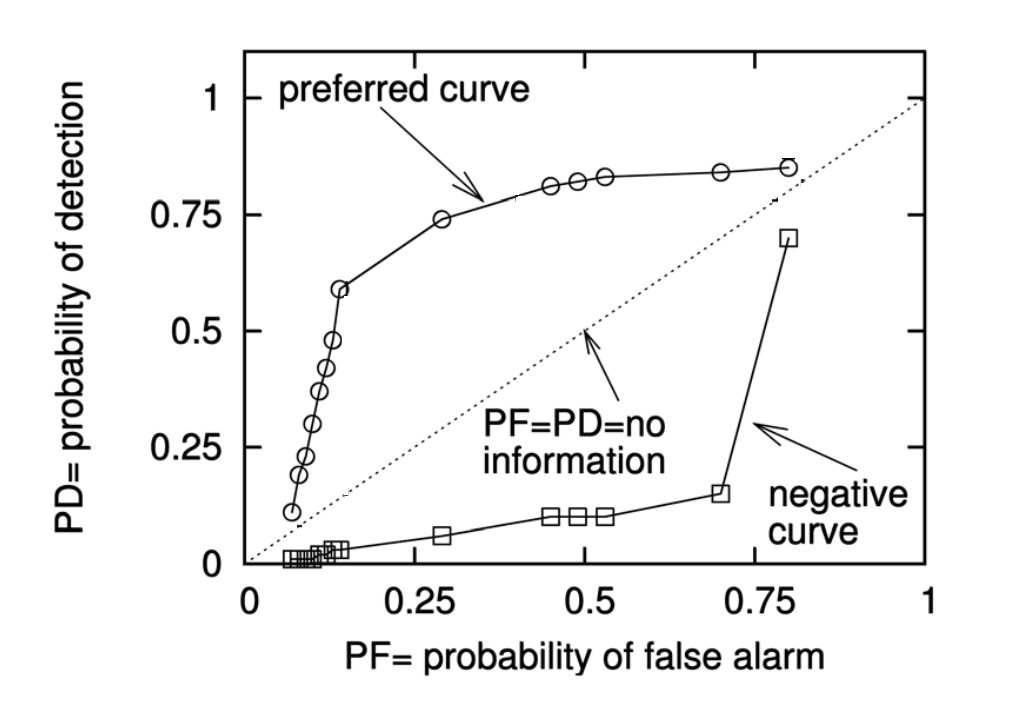
\includegraphics[width=.5\textwidth]{images/ROC.PNG}
	\caption{ نمونه‌ای از نمودار \lr{ROC} \cite{menzies2007data}}
	\label{fig:ROC}
\end{figure}

معیار \lr{AUCEC} معیاری است که تعداد خطوطی از برنامه که  توسط تیم تضمین کیفیت و یا توسعه دهنهده گان نیاز است بررسی و آزموده شود را در نظر می گیرد. ایده ی به موثر بودن از نظر هزینه 
\endnote{Cost-effectiveness}
برای مدلهای پیش بینی خطا برای اولین بار توسط آریشلم و همکاران \cite{arisholm2007data} ارائه گردید. موثر بودن از نظر هزینه به این معنا است که چه تعداد خطا با بررسی و یا تست  \lr{$\%n$ } اول خطوط می توان یافت. به عبارت دیگر اگر یک مدل پیش بینی خطا بتواند تعداد خطای بیشتری را با بررسی و تلاش در آزمون کمتر نسبت به باقی مدلها بیابد می توان گفت که تاثیر آن از نظر هزینه بیشتر است. دو منحنی در  قسمت راست شکل \ref{fig:AUCEC} برای دو مدل پیش بینی مختلف آمده است. هر دو مدل دارای سطح زیر نمودار یکسانی هستند اما زمانی که 20\lr{\%}  اول محور افقی در نظر گرفته می شود مدل \lr{x}  کارایی بهتری دارد. نمودار سمت چپ مدلهای تصادفی، عملی و بهینه را نشان می دهد.

\begin{figure}[H]
	\centering
	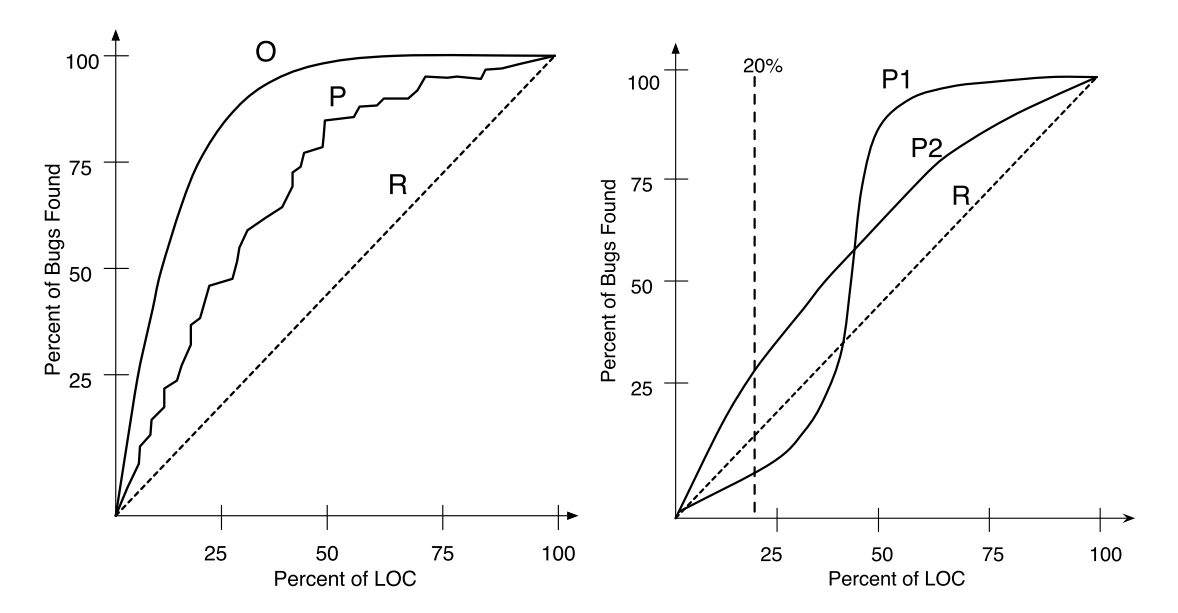
\includegraphics[width=.7\textwidth]{images/AUCEC.PNG}
	\caption{ نمودار موثر بودن از نظر هزینه \cite{rahman2011bugcache}}
	\label{fig:AUCEC}
\end{figure}
